\documentclass[12pt,a4paper,titlepage,headinclude,bibtotoc]{scrartcl}

%---- Allgemeine Layout Einstellungen ------------------------------------------

% Für Kopf und Fußzeilen, siehe auch KOMA-Skript Doku
\usepackage[komastyle]{scrpage2}
\pagestyle{empty}
\setheadsepline{0.5pt}[\color{black}]
\automark[section]{chapter}


%Einstellungen für Figuren- und Tabellenbeschriftungen
\setkomafont{captionlabel}{\sffamily\bfseries}
\setcapindent{0em}


%---- Weitere Pakete -----------------------------------------------------------
% Die Pakete sind alle in der TeX Live Distribution enthalten. Wichtige Adressen
% www.ctan.org, www.dante.de

% Sprachunterstützung
\usepackage[ngerman]{babel}

% Benutzung von Umlauten direkt im Text
% entweder "latin1" oder "utf8"
\usepackage[utf8]{inputenc}

% Pakete mit Mathesymbolen und zur Beseitigung von Schwächen der Mathe-Umgebung
\usepackage{latexsym,exscale,stmaryrd,amssymb,amsmath}


\usepackage[nointegrals]{wasysym}
\usepackage{eurosym}

% Anderes Literaturverzeichnisformat
%\usepackage[square,sort&compress]{natbib}
\usepackage{hyperref}
% Für Farbe
\usepackage{color}
\usepackage{graphicx}
\usepackage{wrapfig}
\usepackage{subfigure}

% Caption neben Abbildung
\usepackage{sidecap}

% Befehl für "Entspricht"-Zeichen
\newcommand{\corresponds}{\ensuremath{\mathrel{\widehat{=}}}}
% Befehl für Errorfunction
\newcommand{\erf}[1]{\text{ erf}\ensuremath{\left( #1 \right)}}

%Fußnoten zwingend auf diese Seite setzen
\interfootnotelinepenalty=1000

%Für chemische Formeln (von www.dante.de)
%% Anpassung an LaTeX(2e) von Bernd Raichle
\makeatletter
\DeclareRobustCommand{\chemical}[1]{%
  {\(\m@th
   \edef\resetfontdimens{\noexpand\)%
       \fontdimen16\textfont2=\the\fontdimen16\textfont2
       \fontdimen17\textfont2=\the\fontdimen17\textfont2\relax}%
   \fontdimen16\textfont2=2.7pt \fontdimen17\textfont2=2.7pt
   \mathrm{#1}%
   \resetfontdimens}}
\makeatother

%Honecker-Kasten mit $$\shadowbox{$xxxx$}$$
\usepackage{fancybox}

%SI-Package
\usepackage{siunitx}

%keine Einrückung, wenn Latex doppelte Leerzeile
\parindent0pt

%Bibliography \bibliography{literatur} und \cite{gerthsen}
%\usepackage{cite}
\usepackage{babelbib}
\selectbiblanguage{ngerman}

\begin{document}

\begin{titlepage}
%\centering
%\textsc{\Large Praktikum zur Einführung in die physikalische Chemie,\\[1.5ex] Universität Göttingen}

\vspace*{3cm}

\rule{\textwidth}{1pt}\\[0.5cm]
{\huge \bfseries
  Interferenz\\[1.5ex]
  und Wellenlängenmessung}\\[0.5cm]
\rule{\textwidth}{1pt}

\vspace*{3cm}

\begin{Large}
\begin{tabular}{ll}
Durchführende: &  Alea Tokita\\
Versuchspartner: &  Julia Stachowiak\\
Assistentin: & Annemarie Kehl\\
 Versuchsdatum: & 09.11.2015\\
 Datum der Abgabe: & 16.11.2015\\
\end{tabular}
\end{Large}

\vspace*{0.8cm}

%\begin{Large}
%\fbox{
  %\begin{minipage}[t][2.5cm][t]{6cm} 
   % Eingegangen am:
  %\end{minipage}
%}
%\end{Large}

\end{titlepage}

\tableofcontents

\newpage



\section{Theorie}

\section{Experimentelles}

\subsection{Versuchsaufbau}

\subsubsection{Skizze der Apperatur}
\begin{figure} [h]
\begin{center}
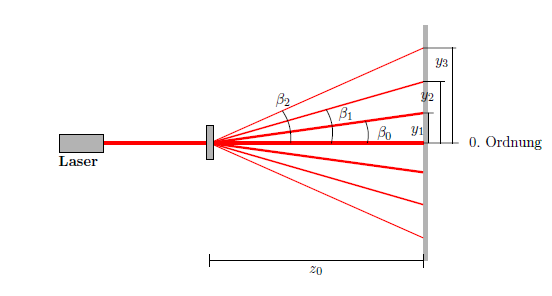
\includegraphics[scale=1]{Versuchsaufbau.png} \end{center}
\caption{Versuchsaufbau}
\end{figure}

Zunächst wird der Versuch wie auf der Skizze beschrieben aufgebaut.
Ein Laser strahlt auf ein Siebgitter, wodurch auf einem sich dahinter befindenden, an ein Holzrahmen befestigtes, Milimeterpapier ein Interferenzmuster entsteht. Anschließend wird das Siebgitter durch ein anderes Siebgitter, nun unbekannter Gitterkonstante, ersetzt.


\subsection{Durchführung}
Die entstehenden Beugungsmuster werden auf das Papier übertragen. Dabei werden jeweils die drei Punkte  oberhalb und unterhalb des nullten Beugunsmaximum übertragen.
Das Militmeterpapier wird von dem Holrahmen genommen und die Abstände $y_{y},y_{2},y_{3}$ der Punkte oberhalb des nullten Maximum zu diesem und die Abstände $y_{-1},y_{-2},y_{-3}$ unterhalb des nullten Maximum zu diesem gemessen.







\section{Auswertung}

Ja aber am Schluss ist es explodiert!

\section{Fehlerrechnung}
Wir machen keine Fehler.


\section{Fehlerdiskussion}
Das muss man nicht mehr diskutieren.

\subsection{Diskussion systematischer Fehler}



\subsection{Vergleich mit Literaturwerten}


%\textbf{Interferenz und Wellenlängenmessung am 9.11.2015} \\

%Name: Julia Stachowiak \\
%Versuchspartner: Alea Tokita \\
%Assistentin: \\ \\



%\begin{table}
%\centering
%\begin{large}

%\end{large}
%\begin{tabular}{|p{4 cm}||p{4 cm}|p{4 cm}|}
  %      \hline
   %       Abstand  & Gitter 1  & Gitter 2 \\
    %      \textit{in cm} & & \\
         
         
     %    \hline 
      %   $y_3 $& & \\
      %   \hline
      %   $y_2 $& & \\
      %   \hline
      %   $y_{1} $& & \\
         
      %   \hline
      %   $y_{-1}$& & \\
      %   \hline
      %   $y_{-2}$& & \\
       %  \hline             
       %  $y_{-3}$& & \\
     %    \hline
%\end{tabular}
%\end{table}


\end{document}


